%%%%%%%%%%%%%%%%%%%%%%%%%%%%%%%%%%%%%%%%%%%%%%%%%%%%%%%%%%%%%%%%%%
\section{Introduction}\label{intro}

% Why are we studying this problem
Earthquakes can cause great damage to human society through soil
rupture, movement, tsunami, etc. Some recent earthquakes that
highlight this destructive potential are the great East Japan
Earthquake of 2011 (depicted in figure\ref{GreatEastJapan}), and the
April 2015 earthquake in Nepal. One important tool for the enactment
of policies that minimize the consequences of these events are
earthquake occurrence models (also called risk models). These models
can be used to identify patterns in the seismic mechanisms that
generate earthquakes, and are important to increase our understanding
of these events.


% \cite{ecta14} opening image. Would be better to have a clustered one.
\begin{figure}[]
\centering
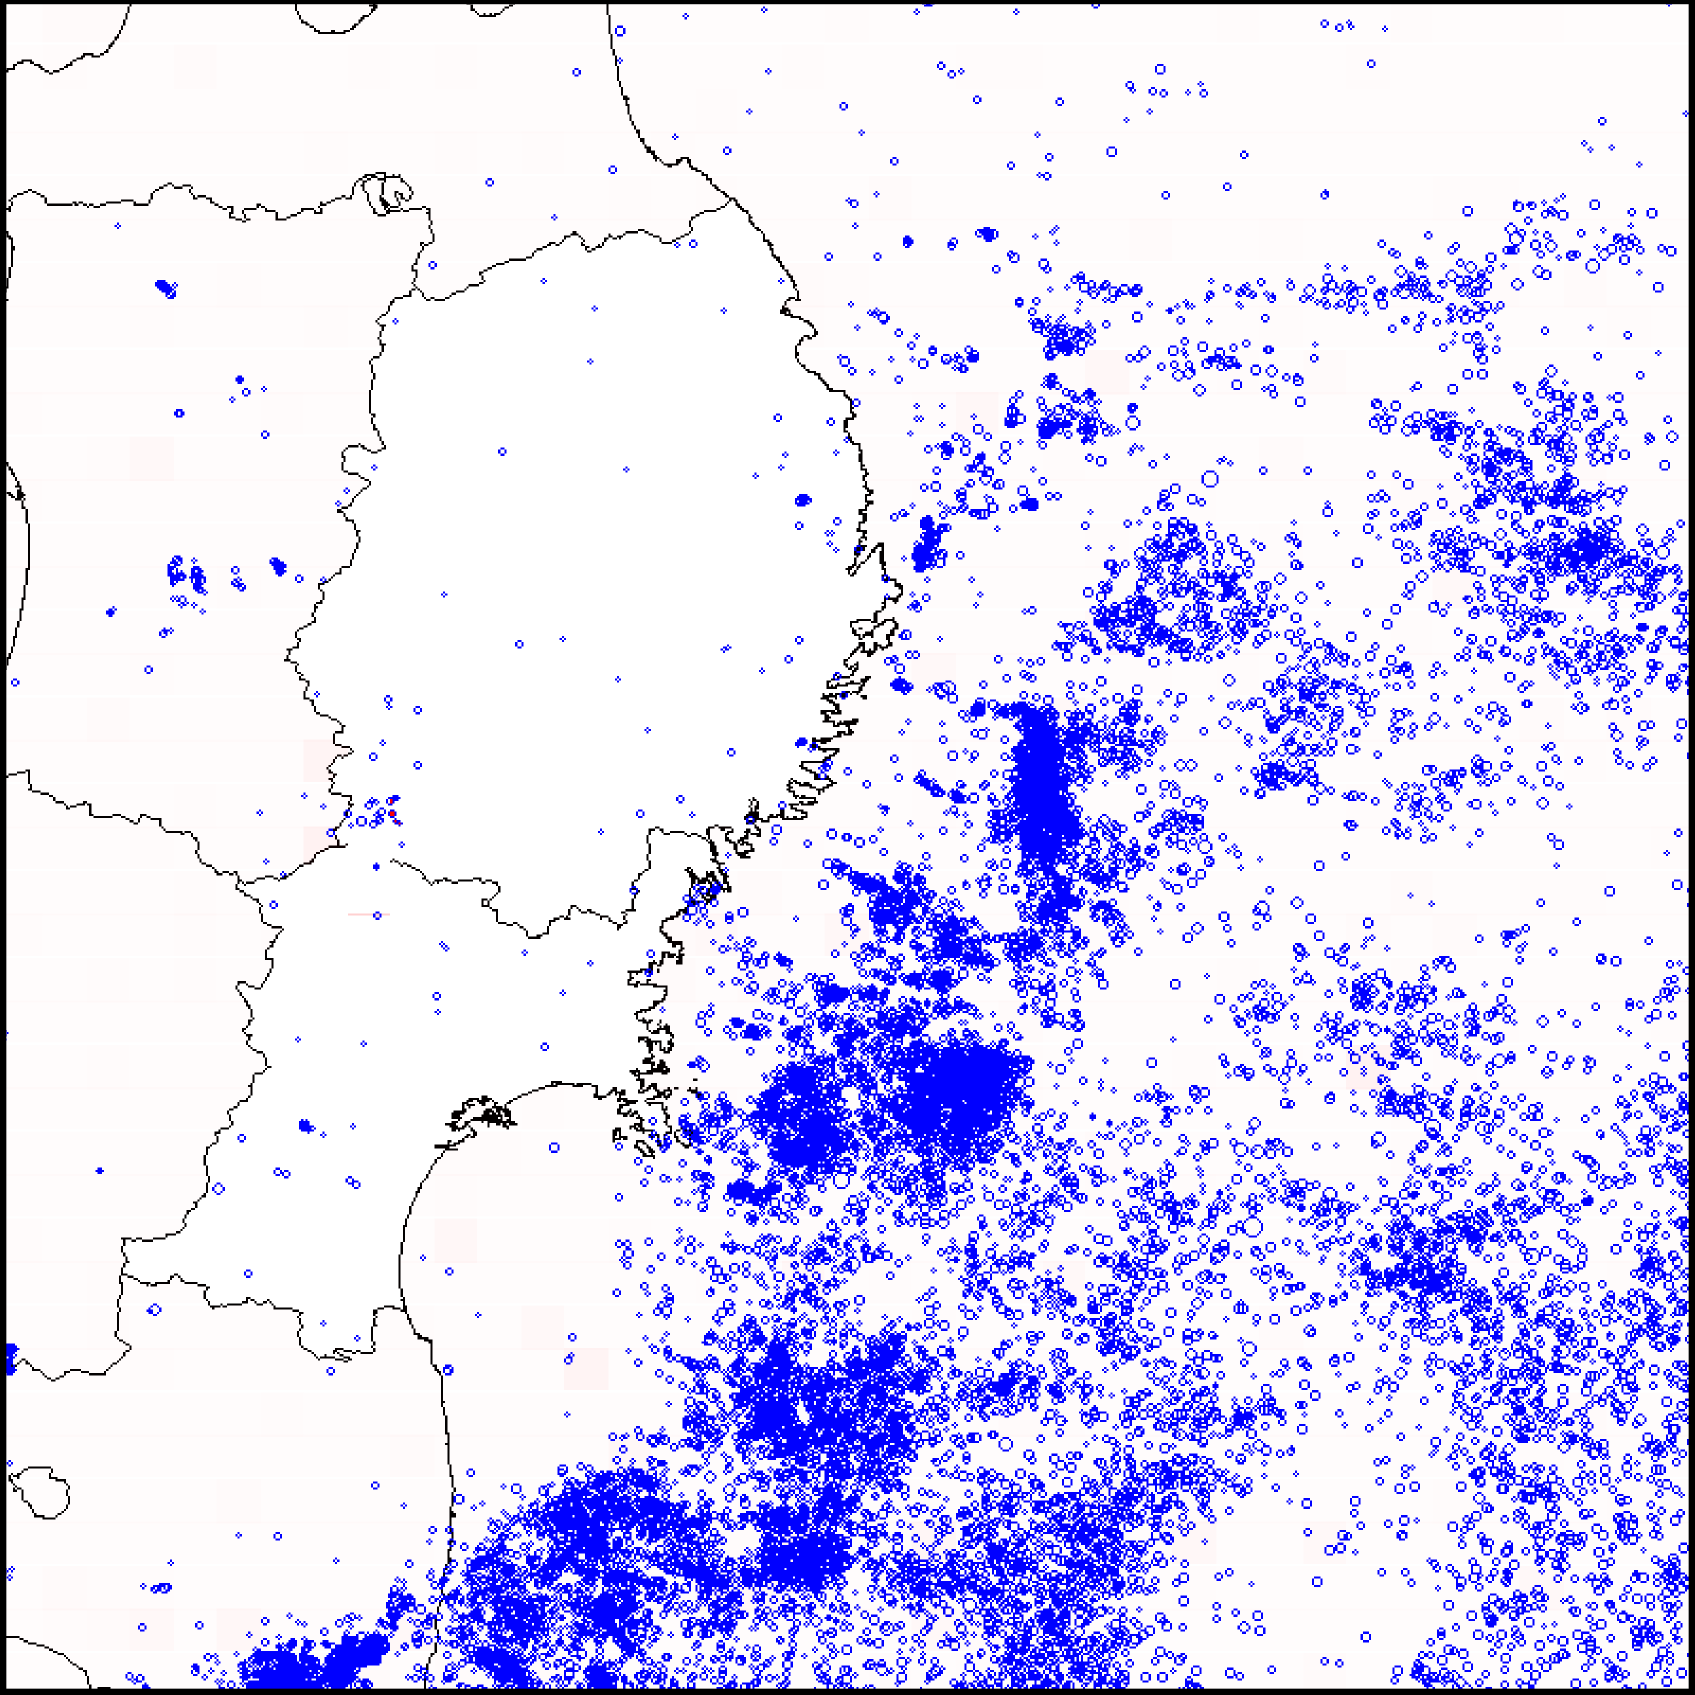
\includegraphics[width=.45\textwidth]{img/earthquakes2011.png}
\caption{Seismic Activity in Eastern Japan in 2011. Each blue dot
  represents one earthquake}
\label{GreatEastJapan}
\end{figure}

% Gabriel's image, does not look very good.
%\begin{figure}[]
%	\centering
%	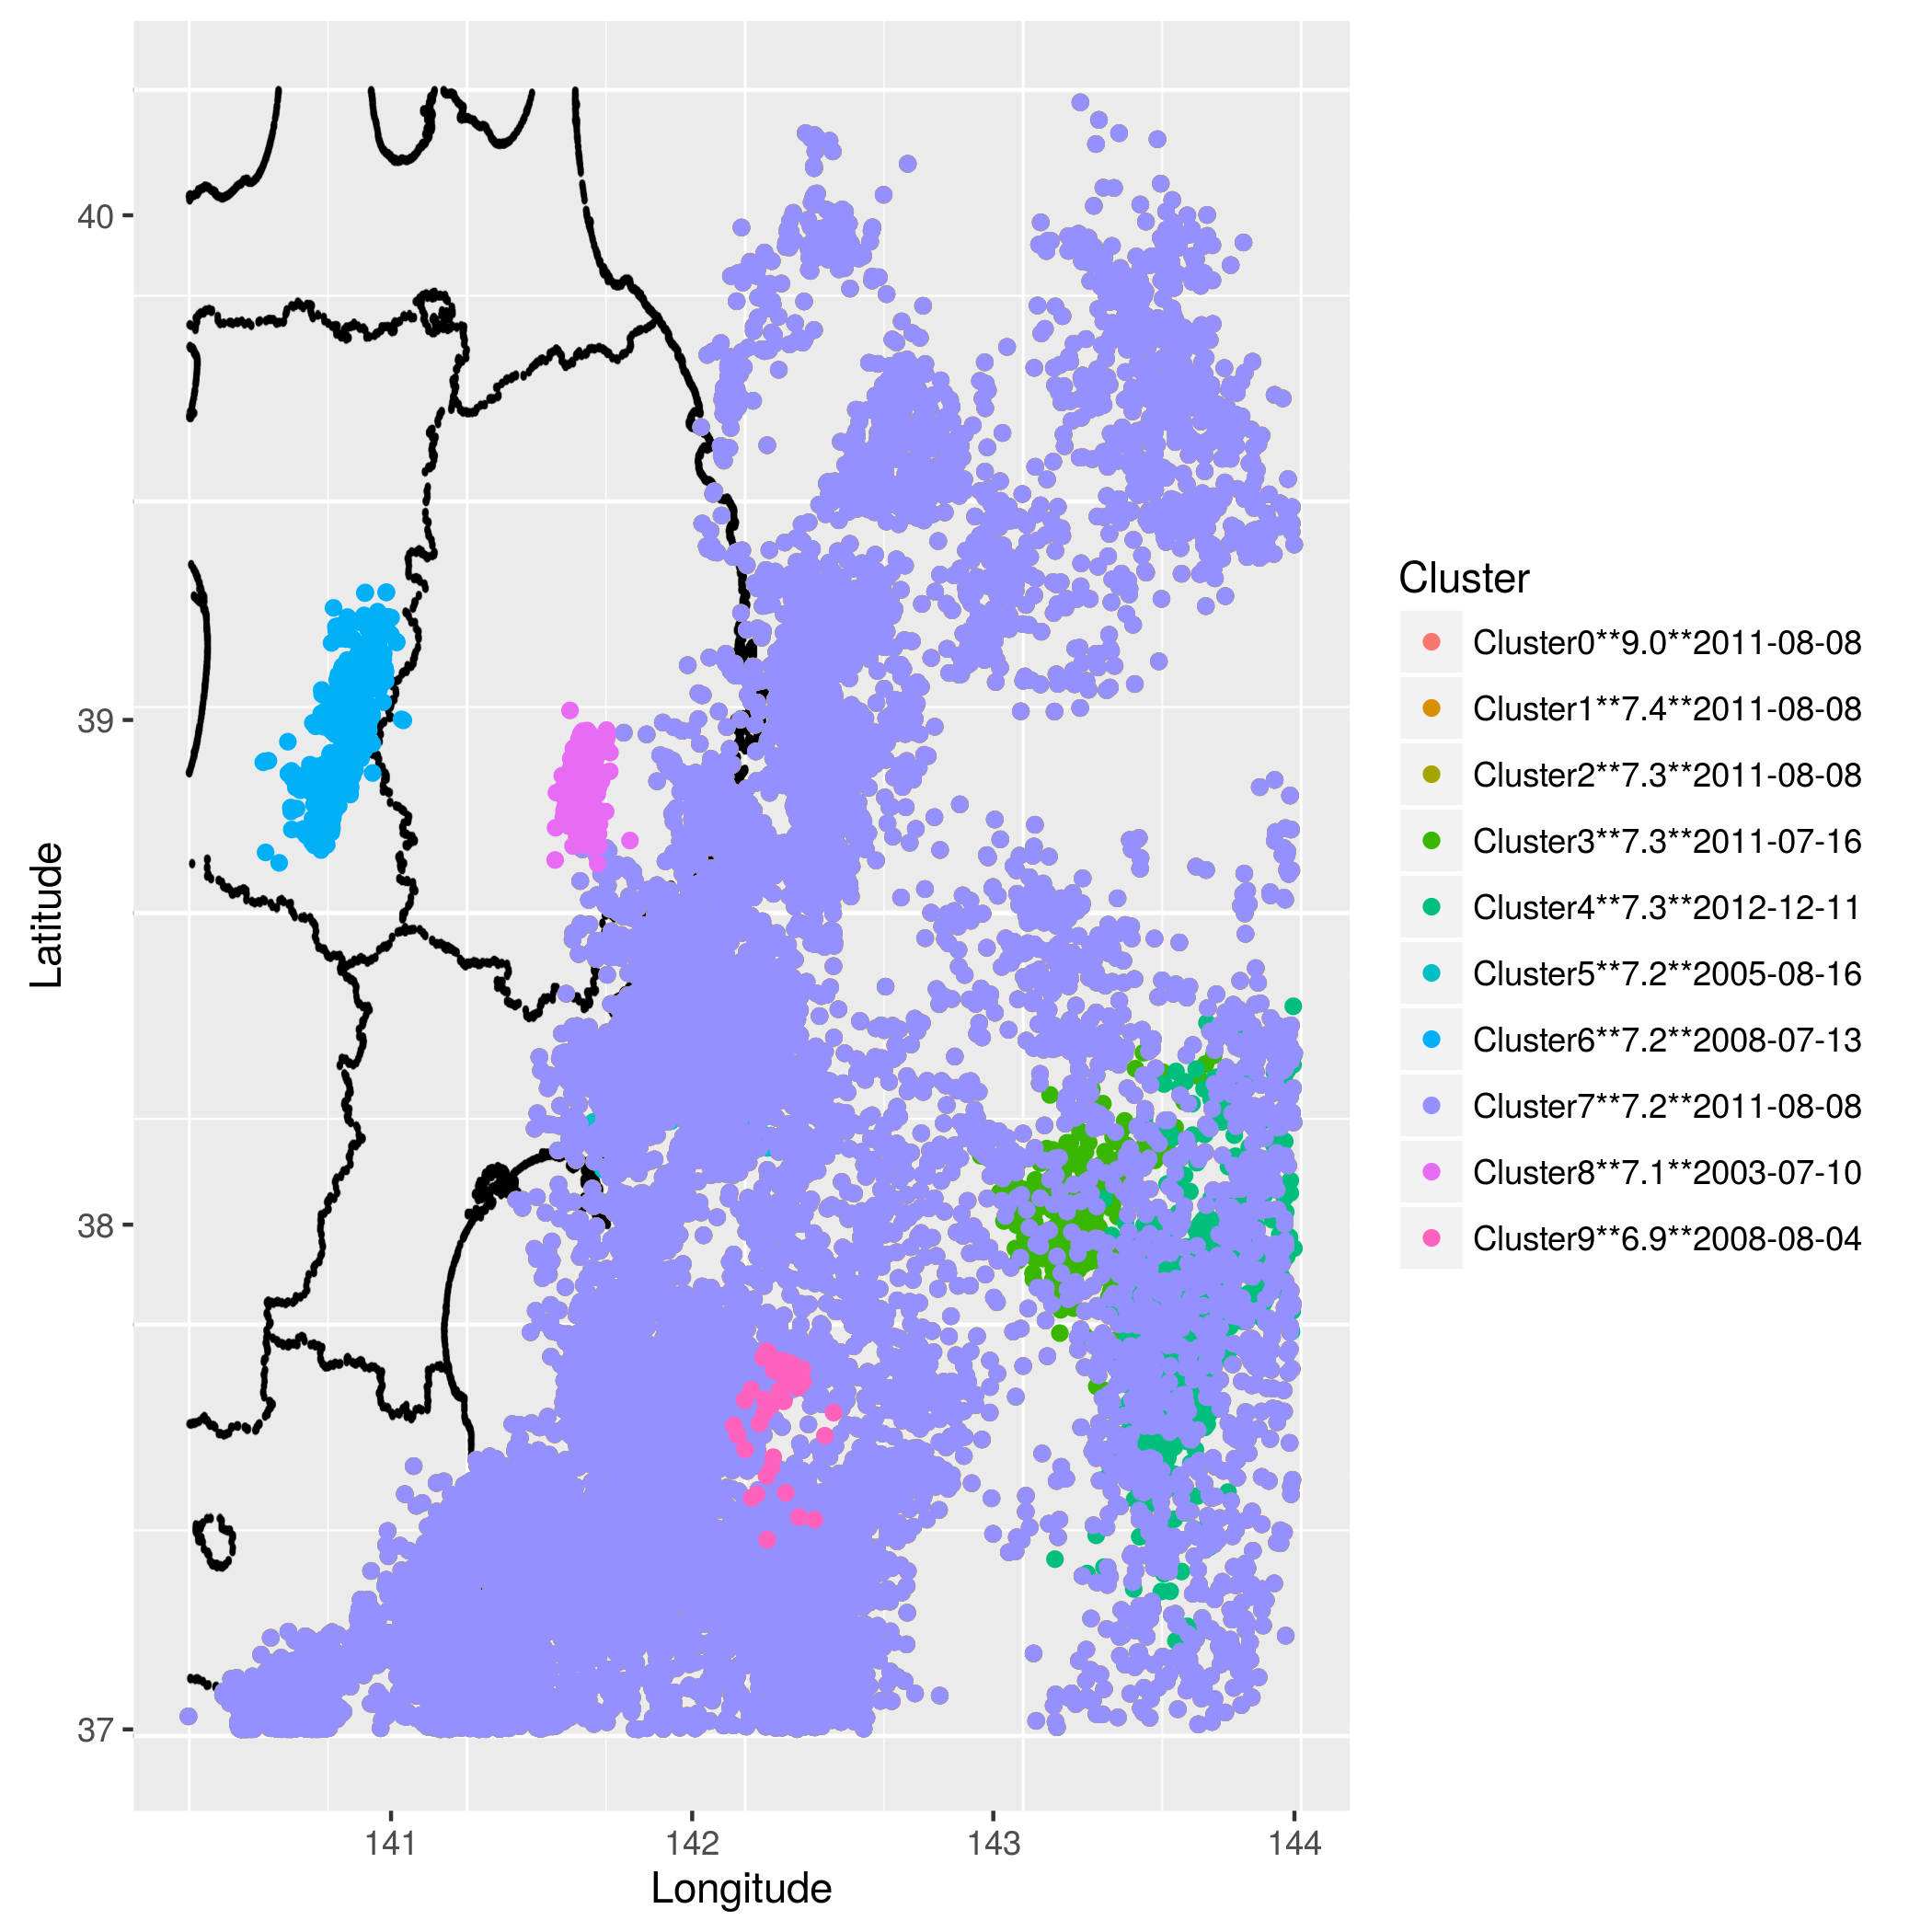
\includegraphics[width=.55\textwidth]{img/slc_leste.png}
%	\caption{Seismic Activity in Eastern Japan during the years of 2003 to 2011.}
%	\label{GreatEastJapan}
%\end{figure}

% Context of our work
In our previous work~\cite{ecta14}, we proposed a way to generate
earthquake risk models using a standard Genetic Algorithm (here called
the GAModel). The GA model was shown to be competitive with the
Relative Intensity (RI) model, while not using any a-priori
information about the distribution of earthquake occurrences. We
summarize the GAModel, and other relevant literature, in
Section~\ref{estadoArte}. However, we have identified two key issues
with the GAModel. Addressing these issues will be the focus of this
paper.

% Ideia and contribution: First issue, representation was too sparse.
% TODO: the non contribution of the parameters is evidenced by the
% random noise of the parameters. It might be good to approach this in
% section 2.
The first issue is that the genome representation used by GAModel has
too many parameters (over 2000 for regular cases). Even though a
majority of these parameters do not contribute for the accuracy of the
final risk model, the size of the search space implies a slower
optimization time. To address this issue, we propose a new genome
representation for an earthquake risk model, which we call
ReducedGAModel. In the ReducedGAModel, only areas with minimal
probability of an earthquake are represented as parameters in the
evolutionary process. By reducing the search space, this
representation is expected to also increase the convergence speed of
the evolutionary optimization process.

% Second issue: Hybridization with domain knowledge
The second issue is that GAModel does not take into account any sort
of domain knowledge, such as the assumption that earthquakes cluster
in both time and space. Heuristic search methods such as Genetic
Algorithms usually benefit from the introduction of domain knowledge
to the search. Therefore, we propose a hybrid version of the GAModel
which incorporates seismic models of earthquake decay. This version,
named Emp-GAModel (Empiric GA Model), generates a model with a much
smaller number of earthquakes than the regular GAModel. For each
earthquake in this model, a sequence of aftershocks is generated using
an adaptation of the Epidemic Type Aftershock Sequence model
(ETAS). We expect that this hybrid approach will produce more accurate
models.

The two proposed adaptations are described in detail in
Section~\ref{Models}. To analyze their contributions, we perform a
simulated comparison of the GAModel, the ReducedGAModel, the
EMP-GAModel, and a combined ReducedEmp-GAModel, which combine both 
adaptations. 

This simulated comparison follows Regional Earthquake Likelihood Model
(RELM) framework described by the Collaboratory for the Study of
Earthquake Predictability
(CSEP)~\cite{schorlermmer2007earthquake}. This framework dictates the
format of the risk model and the utility function used to evaluate the
quality of a risk model (defined as the log-likelihood of the past
earthquake occurrence data given the model). The data used in the
comparisons is the earthquake occurrence catalog from the Japanese
Meteorological Agency (JMA). We focus on earthquakes occurring in the
Japanese archipelago between 2000 and 2010. The RELM framework is
described in section~\ref{Tests}

% TODO: Need many citations regarding declustering
Furthermore, we examine the effect of ``de-clustering'' a catalog in
the generation of risk models. In seismological jargon,
``de-clustering'' refers to the act of identifying groups of
main shock-aftershock earthquakes, and removing all but the main shocks
from the catalog, which is considered the representative earthquake
for the group. Accordingly, a ``de-clustered'' earthquake catalog is
considered to be easier to study, given that the de-clustering process
removes redundant information. On the other hand, there are some
researchers that do not agree with this idea.

In our experiments, we use three catalogs: one that did not undergo
de-clustering (original catalog), and two de-clustered catalogs,
generated by two different de-clustering methods: Window and Single
Link Cluster. The de-clustering strategies are described in
section~\ref{exp}

Our experimental results, detailed in section~\ref{Results}, indicate
that XXXXXXXXXXXXXXXXXXXXXXX XXXXXXXXXXXXXXXXX XXXXXXXXXXXXXXXXXX
XXXXXXXXXXX XXXXXXXXXXXXXxx XXXXXXXXXXXXXXX. We conclude that YYYYYYY
YYYYYYYYY YYYYYYYYYYYYYYYYYY YYYYYYYYYYYYYYYYYYy YYYYYYYYYYYY.


